\documentclass[../Proposal.tex]{subfiles}
\renewcommand{\baselinestretch}{1.5} 
\usepackage{hyperref}
\usepackage[style = apa]{biblatex}
   \addbibresource{references.bib}
\usepackage{csquotes} % Package for direct quotation
\usepackage{placeins} 
\usepackage{geometry} 
    \geometry{margin=1in} 
\usepackage{amsmath}
\usepackage{graphicx}
\usepackage{indentfirst} % Make sure the first paragraph after a section heading is indented

\begin{document}

\subsection*{Overview of Research Design}

Building on significant advancements in affective psychology and creativity research, this study acknowledges the well-documented synergy between mood states and creative cognition. As described in the literature, frameworks categorizing mood along pleasant-unpleasant and activated-deactivated dimensions have elucidated the intricate relationships between mood induction methods and their cognitive consequences (\cite{siedlecka_experimental_2019}). Coupled with the burgeoning exploration of creativity's multifaceted nature---encompassing definitions, underlying cognitive processes, and diverse assessment tasks (\cite{kaufman_cambridge_2010})---this mutual enrichment has paved the way for both theoretical propositions and empirical validations of the mood-creativity linkage.

Echoing \textcite{kaufman_cambridge_2010}'s call for innovative assessment techniques that more accurately reflect the dynamics of creative thinking, this proposed study aims to advance the debate on the mood-creativity connection by introducing a novel \textit{task-measurement} combination, which leverages both the versatility of drawing tasks to uncover the cognitive underpinnings of creativity and employing state-of-the-art artificial intelligence techniques. Focusing on \textit{domain-general}, \textit{little-c} creativity, our study aims to capture the nuanced effects of mood on creative processes and, more specifically, the (potential) building effects of positive mood states on thought-action repertoires (\cite{fredrickson_role_2001}). By distinguishing positive mood states varying on the activation dimension---happiness (high activation) and calmness (low activation), this study seeks to scrutinize the hypothesized flexibility pathway (as suggested by \textcite{de_dreu_hedonic_2008}'s dual pathway to creativity model) in which positive activating mood states, rather than positive deactivating ones, predict cognitive flexibility, characterized by employing wide-ranging and comprehensive cognitive categories to form associations. The conducive influence of positive (activating) mood is further hypothesized to enhance the originality aspect of creativity (i.e., the uncommonness of ideas, solutions, or products). 

Specifically, by adopting validated experimental mood induction methods (\cite{siedlecka_experimental_2019}), this study will explore the effects of positive mood states---ranging from activating to deactivating---on the flexibility pathway of creativity. This research will utilize tasks that not only track the dynamics of creative processes, but also incorporate novel methodologies from generative sketch modeling and NLP to examine the proposed building effects of positive mood states on thought-action repertoires (\cite{fredrickson_role_2001}). The following research questions will guide the investigation:
\begin{enumerate}
    \item How do positive moods across the spectrum of activation level, including positive moods with high level of activation (e.g., happiness) and positive moods with low level of activation (e.g., calmness), affect cognitive flexibility during the creative ideation process, respectively?
    \item How does cognitive flexibility during the creative ideation process further influence the originality aspect of creativity in the final product (i.e., whether flexibility mediates the relationship between positive mood and the originality aspect of creativity)?
\end{enumerate}

Following \textcite{barbot_dynamics_2018}'s Multi-Trial Creative Ideation (MTCI) framework (featuring multi-stimuli approach \& dynamics of ideation process), this proposed study will adopt drawing tasks (particularly the incomplete shape drawing task) and narrative about creative ideation processes to not only record the final creative output, but also track the dynamics of creative thinking that leads to the final completed drawings. The primary contribution of this study is its integration of drawing tasks with deep learning and natural language processing techniques to quantitatively assess both the flexibility and originality aspects of creativity. This method offers a more comprehensive analysis than previous studies that relied solely on verbal tasks such as the alternative use task and the remote association task (e.g., \cite{kenett_investigating_2014}; \cite{kenett_flexibility_2018}) to quantify the flexibility aspect of creativity. Complementing the predominance of verbal creativity assessments with visual creativity (a canonical form of creative expression; \cite{morrisskay_evolution_2010}) allows for a holistic understanding of creative processes. Verbal and visual creativity engage different cognitive and neural pathways; verbal creativity often relies on language-based processes and abstract thinking (\cite{benedek_create_2014}), while visual creativity engages spatial reasoning and visual-motor coordination (\cite{schlegel_artist_2015}). By studying both aspects, this proposed study could uncover complementary insights into the cognitive mechanisms underlying the flexibility aspect of creativity. This integrative approach enhances the validity of the measurements by capturing a broader range of creative expression and providing a more nuanced understanding of the dynamics of creative thinking. Meanwhile, when it comes to assessing the originality aspect of creativity (especially visual creativity), using automated scoring methods effectively addresses several practical limitations in creativity research. These include the high labor costs associated with manual evaluations and the inherent subjectivity that can bias expert ratings (\cite{patterson_audra_2023}). Automated methods provide a scalable and consistent way to evaluate originality, ensuring that the assessments are objective and replicable across different studies.

Specifically, this study will measure flexibility using the Compositional Stroke Embedding (CoSE) model, which utilizes a Gaussian Mixture Model (GMM) to predict potential strokes in the incompleteness shape drawing task. This approach assesses the uncertainty and variability between possible strokes, employing metrics such as entropy and Bhattacharyya distance to capture the dynamic range of creative options. Complementing this, flexibility will be further evaluated through Divergent Semantic Integration (DSI), which employs BERT-generated embeddings to analyze how participants integrate divergent ideas into their narratives. Meanwhile, originality will be evaluated using the Automated Drawing Assessment (AuDrA) model trained with human ratings on the same incompleteness shape drawing task. Together, this proposed study not only aims to elucidate mood-creativity linkage, but also underscores the transformative potential of integrating artificial intelligence into the study of complex human cognitive processes. Together, the overall research design is illustrated in Figure \ref{fig: Overview of Research Design}.

\begin{figure}
    \centering
    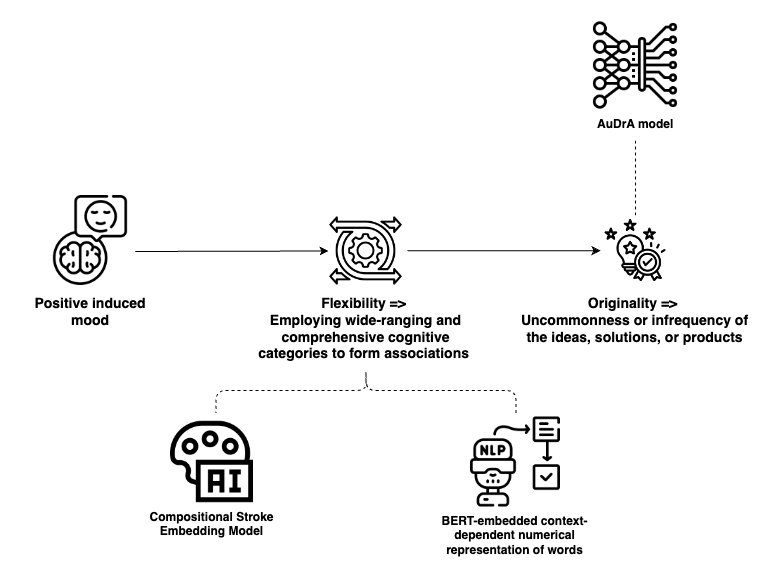
\includegraphics[width=0.8\linewidth, keepaspectratio]{drawio/Overview of Research Design_Full.png}
    \caption{Overview of Research Design}
    \label{fig: Overview of Research Design}
\end{figure}

\subsection*{Experiment Implementation}
The proposed study will design a website to facilitate an online experiment to collect data to test the proposed flexibility pathway linking positive activating mood with the originality aspect of creativity\footnote{See this \href{https://github.com/cty20010831/incomplete_drawing_task}{\textcolor{blue}{public repository}} for more details about the code behind the website.}. As shown in Figure \ref{fig: Workflow of Online Experiment}, this proposed study will first design the experiment using jsPsych (\cite{leeuw_jspsych_2023}), a JavaScript framework to design behavioral experiments running on a web browser. The website will then be pretested among a sample of approximately 30 Amazon Mechanical Turk (MTurk) workers and ask for feedback on areas of improvement regarding the website and research design. Once the final experimental design is finalized, this study plans to recruit approximately 100 participants recruited from MTurk to participate in this online experiment hosted on the improved version of the experiment website, which also allows me to download data for later data analysis.

\begin{figure}
    \centering
    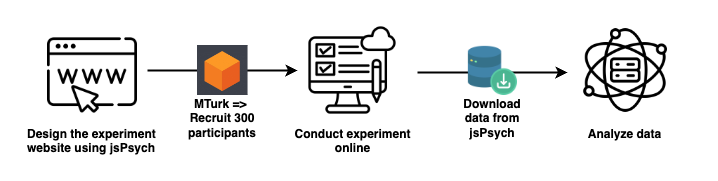
\includegraphics[width=0.8\linewidth, keepaspectratio]{drawio/Workflow.png}
    \caption{Workflow of Online Experiment}
    \label{fig: Workflow of Online Experiment}
\end{figure}

When it comes to the design of the web page in particular, this experiment website will consist of four main blocks: mood induction, incompleteness drawing tasks, narrative on thought processes behind completing the drawings, and survey data collection (see Figure \ref{fig: Experiment Web Page Design}). Specifically, after completing informed consent, participants will undergo mood induction by streaming film clips, which has been proven to be an effective mood induction technique to engage visual and auditory modalities and simulate real-life emotional situations (\cite{siedlecka_experimental_2019}). After controlling display size and film duration, this proposed study will play video clips that target different induced mood states for the three randomly assigned groups. Specifically, amusing and engaging clips from validated sets (e.g., Sister Act; \cite{maryam_fakhrhosseini_affectemotion_2017}) will be used to induce happiness, while calmness will be elicited using stimuli suggested by \textcite{kimura_emotional_2019}. For the control group, neutral clips such as nature documentaries and weather news will be chosen (\cite{siedlecka_experimental_2019}). Before viewing the video clips, participants will receive the instruction to immerse themselves in the clip as they would when watching a movie in a cinema, without needing to memorize any details from the clips they will be watching. This way, the framing effects on induced moods could be minimized, as opposed to using more directive prompts like ``Let yourself experience your emotions fully.'' Furthermore, the Self Assessment Manikin (SAM; \cite{bradley_affect_1999}), a graphic figure representing the valence and arousal elements in mood states, will be used to check the effectiveness of mood induction based on participants' valence and arousal ratings (\cite{kucera_using_2012}).

\begin{figure}
    \centering
    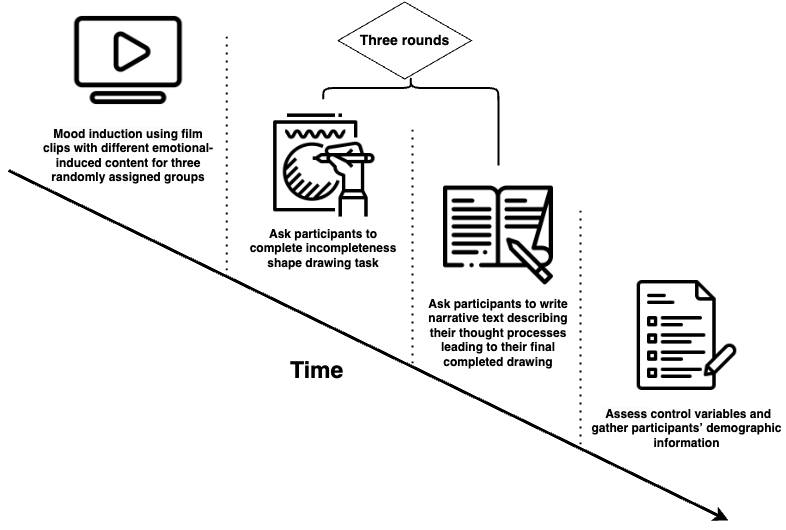
\includegraphics[width=0.7\linewidth, keepaspectratio]{drawio/Experiment Timeline.png}
    \caption{Experiment Web Page Design}
    \label{fig: Experiment Web Page Design}
\end{figure}

The next section of the experiment website is the creative task of incompleteness shape drawing task, where participants will be presented with an abstract or concrete shape and asked to creatively integrate this initial shape into their drawings at their own pace (see Figure \ref{fig: Example of Incompleteness Shape Task}; \cite{patterson_audra_2023}). To implement this drawing task, this study will develop a web-based drawing interface using \textit{sketchpad} plugin of jsPsych (\cite{leeuw_jspsych_2023}). This plugin includes options for undoing, redoing, and clearing strokes. In addition, it records the position (x, y coordinates) and the timing of mouse movements during drawing and saves images as text (json-like structure) using base64 encoding for later data analysis (\cite{bainbridge_tutorial_2022}). Participants will be told to use their imagination to finish the drawing in any way they like and take their time and to be as creative as possible. After each drawing session, participants provide a detailed narrative describing their approach to the incomplete shape, including initial impressions, specific ideas or associations, and any shifts in direction during the process. They reflect on thematic elements such as nature, technology, or abstract concepts, as well as any emerging themes and decisions guiding their creative choices. This narrative captures their thought processes, offering insights into the cognitive mechanisms influencing their creativity. There will be in total three rounds of incompleteness drawing task (different starting incomplete shapes) and narrative on thought processes, echoing \textcite{barbot_dynamics_2018}'s multi-stimuli approach to uncover the (variation of) the dynamics behind creative thinking.

The final section asks participants to complete survey questions related to control variables and demographics. For starters, participants will complete several questionnaires that measure control variables in this study, including trait affectivity (measured by Positive and Negative Affect Schedule; \cite{watson_development_1988}), openness to experiences (measured by the Ten Item Personality Measure; \cite{gosling_very_2003}), cognitive flexibility (measured by Cognitive Flexibility Scale; \cite{martin_new_1995}), and self-rated artistic skill. Afterwards, they will provide demographic information, including age, gender, race, and education level. 
\begin{figure}
    \centering
    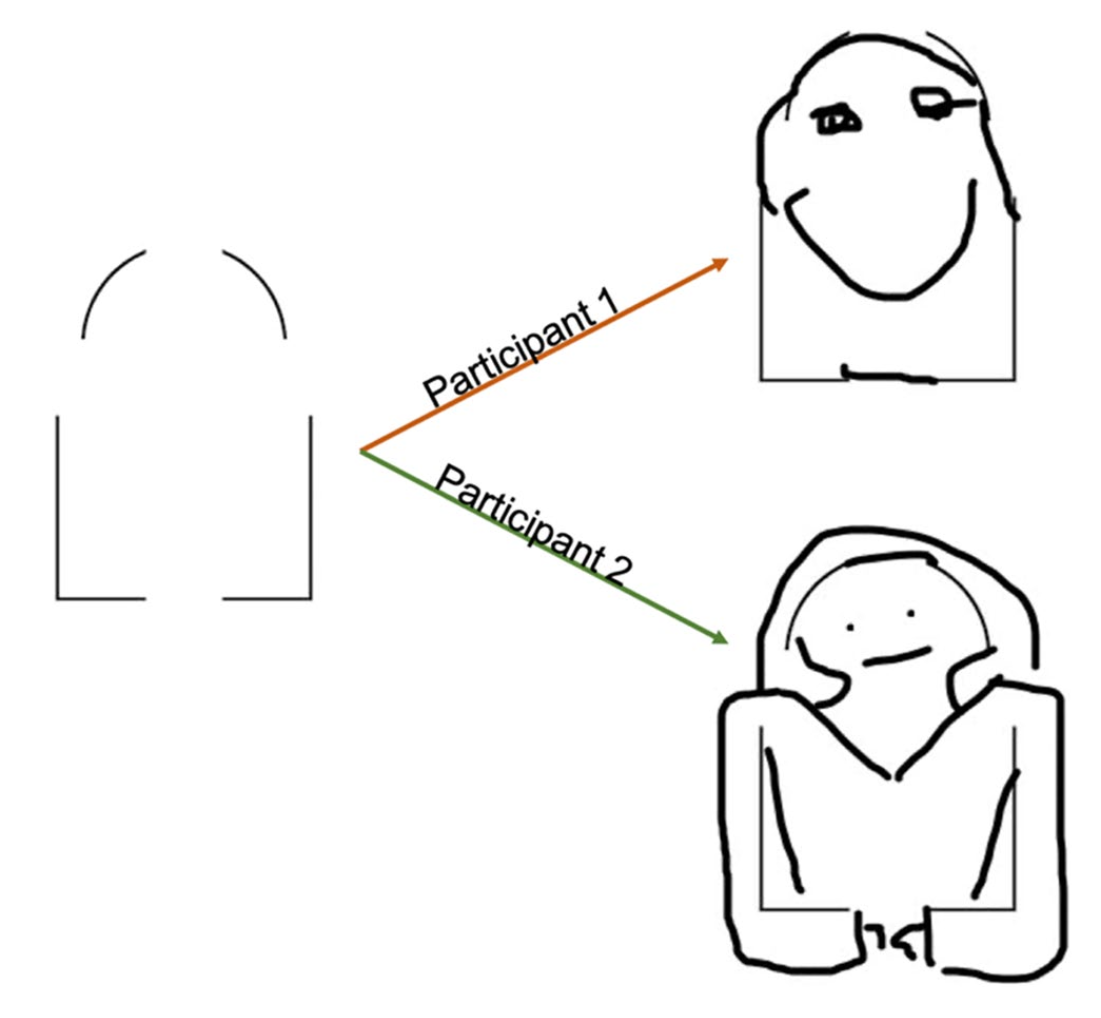
\includegraphics[height=0.2\textheight, keepaspectratio]{screenshots/Example_Incompleteness_Shape.png}
    \caption{Example of Incompleteness Shape Task}
    \label{fig: Example of Incompleteness Shape Task}
\end{figure}

\subsection*{Methods}

\subsubsection*{Measuring the Flexibility Aspect of Creativity}
This proposed study will investigate the flexibility pathway leading to creativity using the incompleteness shape drawing task. The flexibility pathway refers to the process of employing wide-ranging and comprehensive cognitive categories to form associations, according to \textcite{nijstad_dual_2010}'s dual pathway to creativity model. In the context of the incompleteness shape drawing task, flexibility specifically refers to the ability of participants to explore a wide range of qualitatively distinct creative solutions (both in terms of starting position and trajectory) for each stroke they add to an incomplete shape. This operational definition of flexibility hinges on the premise that a more creatively flexible individual will not only consider a broader array of potential next strokes, but also open to the possibility of choosing other paths that are qualitatively distinct from each other in their choice space during their creative processes.

\paragraph*{Compositional Stroke Embedding Model}
The use of a generative model, specifically the Compositional Stroke Embedding (CoSE) model in this proposed study, allows for a novel examination of the flexibility aspect of creativity by taking advantage of the ability of the model to predict the next stroke using the Gaussian mix model (GMM). Specifically, the model's ability to forecast these strokes with both varying degrees of uncertainty (in its prediction) and between-component (potential stroke) distances offers a tangible metric to assess both the expansiveness and dynamic narrowing of creative possibilities of an individual's creative thought process. Initially, with the canvas largely blank and minimal constraints imposed by previous strokes, the GMM's forecasts encompass a broad spectrum of potential directions. This high degree of uncertainty and between-component distances in the model's predictions mirror an expansive field of creative potential, where participants are poised at the brink of numerous possible creative trajectories. Such a scenario exemplifies the task's capacity to engage a participant's broad and inclusive cognitive categories. As participants engage in the task, each decision—each stroke added to the canvas—serves not just as an act of creation but as a sieve, gradually filtering the boundless array of potential futures into a converging path toward a specific creative outcome. This process is hypothetically reflected in the gradual decrease in degree of uncertainty and between-component distances.

In order to capture the degree of uncertainty and between-components distances in GMM's prediction that are pertinent to the flexibility aspect of the creative ideation process, this proposed study will use the following two measures (see Appendix \ref{appendix: entropy} and Appendix \ref{appendix: bhattacharyya distance} for details in formula): 
\begin{enumerate}
    \item \textbf{Entropy of the Gaussian Mixture Model (GMM)}. Entropy quantifies the uncertainty or variability in the model predictions for the next stroke. High entropy indicates a state of high creative flexibility, where the participant is free to explore (and potentially follow) a wide range of directions for their next stroke at a given number of completed strokes. This study adopts the approach proposed by \textcite{huber_entropy_2008} to approximate the entropy of a GMM by incorporating the Kullback-Leibler (KL) divergence between each pair of components within the mixture, as suggested by \textcite{hershey_approximating_2007}. This formulation provides a method for approximating the entropy of a GMM by considering the diversity and weight of each component in the mixture, thus reflecting the variability and uncertainty in the model predictions for the next stroke in the drawing task.
    
    \item \textbf{Bhattacharyya Distance for Measuring Component Divergence}. Another measure to capture the flexibility aspect of creativity in this study is the Bhattacharyya distance, a measure of divergence between two probability distributions. Bhattacharyya distance is a metric of similarity that ranges from 0 to $\infty$, where a smaller value indicates a higher degree of similarity (or overlap) between the two distributions, and a higher value suggests a greater divergence. It is particularly useful in the context of GMM for assessing overlap and separation between different clusters (\cite{alangari_intrinsically_2023}). This measure is instrumental in global interpretation, helping to discern the distinctiveness and similarities between clusters by quantifying the degree of overlap between their corresponding Gaussian components. Taking a step further, the aggregated Bhattacharyya distance in the context of GMM, where multiple Gaussian components represent different aspects of the data (creative possibilities in the context of my study), can be conceptualized as a measure of overall divergence or dissimilarity between all pairs of components within the model. This aggregated measure provides a holistic view of the diversity and separation inherent in the model's representation of the data. In the case of the incompleteness shape drawing task, the aggregated Bhattacharyya distance across all component pairs in the GMM provides a quantitative measure of the dynamic narrowing process of possibilities of next stroke (positions and trajectories). A decrease in aggregated Bhattacharyya distance over time would indicate a gradual focusing of creative possibilities, reflecting the participant's transition from exploring a wide array of potential ideas to honing in on a more defined set of creative directions. 

\end{enumerate}

The interplay between the entropy and the Bhattacharyya measure as quantitative tools offers a nuanced view of the creative journey in the drawing task. Initially, one might expect both high entropy (indicating many possible next strokes) and significant distances between GMM components (suggesting diverse creative paths). Initially, high values in these measures reflect a phase of creative exploration, where participants are most open to employing a wide array of cognitive categories and making remote associations. As the task progresses, both measures are likely to decrease, reflecting the natural progression of creative work from exploration to execution. This progression from a broad, unbounded exploration of ideas towards a more focused and refined output is at the heart of cognitive flexibility. By quantifying this transition, the proposed measures not only capture the essence of the flexibility aspect of creativity, but also provide a structured means to examine how individuals navigate the complex landscape of potential ideas. For instance, the rate at which the possibility space narrows (as captured by these measures) mirrors the cognitive shifts that occur as a creative work evolves, offering a direct link between the theoretical underpinnings of cognitive flexibility and its practical, observable manifestations in creative tasks.

As such, investigating both the overall characteristics and the dynamic trend of the entropy of GMM and aggregated Bhattacharyya distance enables a nuanced view of the creative journey in the incompleteness shape drawing task for each participant. This is not limited to overall aggregated measure of the entropy of GMM and aggregated Bhattacharyya distance but also the steepness of the trend and the frequency and timing of significant rate of change (inflection point) of these measures over time. Here are three measures that I believe effectively distinguish the flexibility pathway during one's creative ideation process (i.e., higher flexibility versus lower flexibility aspect of creativity):
\begin{enumerate}
    \item \textbf{Average Entropy of GMM and Aggregated Bhattacharyya Distance Across Trials}. Since the entropy of GMM indicates the level of uncertainty in the model's prediction of the participants' next move(s), a higher average entropy signifies a broader and meanwhile unpredictable exploration within the creative process, a hallmark of heightened cognitive flexibility. This is complemented by a larger aggregated Bhattacharyya distance, which underscores the extent of divergence in the exploration of creative possibilities, reflecting an engagement with a broad spectrum of cognitive categories. Hence, calculating these aggregated measures for each participant enables us to distinguish the overall breadth of creative exploration and levels of creative flexibility.
    \item \textbf{Aggregated Rate of Change in Entropy of GMM and Aggregated Bhattacharyya Distance}. Extending from the average of entropy of GMM and aggregated bhattacharyya distance, the aggregated rate of change in these measures becomes pivotal. Specifically, individuals endowed with a high degree of creative flexibility tend to engage in a more extended period of ideational exploration, evidenced by a slower rate of convergence (a gradual decrease in both entropy and Bhattacharyya distance). This phenomenon is quantified by computing the first derivative of these measures over time, which offers a glimpse into the dynamic interplay between divergent and convergent thinking phases. The direction of this derivative, whether positive or negative, eloquently speaks to the prevailing mode of thought, be it expansive exploration (divergence) or focused refinement (convergence).
    \item \textbf{Number and Timing of Inflection Points}. The algorithmic identification of inflection points (significant shifts in the rate of change) within the creative process, especially when analyzing the entropy of GMM or aggregated Bhattacharyya distance over GMM components in a time series, provides a nuanced view of the level of flexibility in the creative ideation process. First, it is hypothesized that people with high cognitive flexibility might exhibit a greater \textit{number of inflection points}. This pattern suggests a more dynamic process that involves frequent shifts between exploration and refinement, reflecting their comfort with navigating diverse cognitive spaces and their readiness to adapt their creative strategies in response to new insights. Second, when it comes to the \textit{timing of inflection points}, it is posited that the first major inflection point, marking the shift from initial exploration to more focused convergence, might occur later for individuals with high flexibility, suggesting a prolonged engagement with a broad range of possibilities before narrowing down to specific ideas. For this proposed study, I will adopt the Pruned Exact Linear Time (PELT) algorithm (\cite{dorcas_wambui_power_2015}) using \textit{ruptures} Python library (\cite{truong_selective_2020}) to identify the inflection point(s) in the time series of entropy of the GMM and Bhattacharyya distance.
\end{enumerate}

\paragraph*{Narrative about Creative Ideation Processes} 
Apart from capturing the flexibility aspect of creativity using generative stroke models, this study relies on participants' verbal description on their thought processes (behind their completed drawings) as a complementary measure to examine the diversity of ideas/concepts they connect during creative ideation processes. As one type of observation offering data on individuals' cognitive processes (\cite{ericsson_verbal_2003}), verbal report could serve as a window into people's thought processes and the dynamics of creative thinking by requiring the organization and expression of ideas, reflecting the cognitive processes involved in structuring and connecting these ideas. As individuals construct stories, they engage in memory retrieval, association, and synthesis, which are key components of creative thinking. Narratives unfold over time, mirroring the dynamic nature of creative thought, allowing researchers to observe how ideas evolve, merge, and diverge.

Specifically, this study will utilize Divergent Semantic Integration (DSI; \cite{johnson_divergent_2022}) to measure the diversity of concepts participants connected to complete incomplete shapes, inferred through their narrative about how they have approached and completed the drawings. As an original measurement of creativity in narratives, DSI echos \textcite{kaufman_cambridge_2010}'s call for interdisciplinary approaches to measure creativity by integrating \textcite{mednick_associative_1962}'s associative theory with distributional semantics theory in the linguistics field to assess how narratives integrate divergent ideas. On the one hand, DSI captures the essence of creativity featuring forming associations between disparate concepts in memory. On the other hand, DSI capitalizes on the theory of distributional semantics, which allows a computational understanding of semantics (word meanings) in a salable manner. Specifically, distributional semantics is based on the Distributional Hypothesis, which posits that words with similar meanings occur in similar contexts (\cite{lenci_distributional_2008}). By analyzing word co-occurrence in large text corpora, this approach creates vector-based representations of words in a high-dimensional space, and the proximity of these vectors reflects semantic similarity, allowing distributional semantics to capture word meanings based on usage patterns (\cite{boleda_distributional_2020}).

Together, DSI is arguably an effective measure to characterize the flexibility pathway of creativity. By combining associative theory with distributional semantics, DSI captures the association and integration of connections between disparate ideas and concepts---a hallmark of creative flexibility. Furthermore, it employs the BERT model (\cite{devlin_bert_2019}) to generate context-dependent embedding of words to capture nuanced semantic relationships that reflect creative integration (see Appendix \ref{appendix: DSI} for details in formula). This approach provides a precise measurement of the semantic distance of concepts within the concept space that are involved in completing the drawings. Specifically, a more flexible individual would navigate further in his/her concept space to connect more distinct concepts, which predicts a higher DSI.

% After converting narrative texts into BERT word embeddings, pairwise semantic distances are calculated, which are further used to derive DSI scores using the following formula (\cite{johnson_divergent_2022}):
% \begin{equation*}
%             DSI = \frac{2}{n(n-1)} \sum_{i=1}^{n} \sum_{k=i+1}^{n} D_{\text{cos}}(\omega_i, \omega_k)
%         \end{equation*}
%         \begin{equation*}
%             D_{\text{cos}}(\omega, k) = 1 - \frac{\omega \cdot k}{\|\omega\| \|k\|}
%         \end{equation*}
%         where:
%         \begin{itemize}
%             \item \(\omega_i, \omega_k\) are the embeddings for words \(i\) and \(k\).
%             \item \(D_{\text{cos}}\) measures the cosine distance, which is 1 minus the cosine similarity, between the embeddings.
%             \item \(n\) is the number of unique word pairs considered.
%         \end{itemize}

\subsubsection*{Measuring the Originality Aspect of Creativity}
To measure \textit{originality} aspect of creatvity, this study will refer to the pre-trained AuDrA model and implementation code provided on \textcite{patterson_audra_2023}'s \href{https://osf.io/kqn9v/}{open-access repository}. In an attempt to overcome the limitations of subjective creativity scoring, including labor cost and subjectivity, these authors joined the movement to capitalize on machine learning to automatically assess creativity (e.g., \cite{acar_applying_2023}; \cite{beaty_automating_2021}). Targeting at the tablet-based drawing task under \textcite{barbot_dynamics_2018}'s MTCI framework, AuDrA extends the (mere) fluency measurement via reaction time data in the original task by developing an automated method to assess the originality of the sketches.

As a modified ResNet architecture that allows continuous prediction of creativity scores, AuDra model was trained using over 13,000 sketches rated for creativity by nearly 60 human raters across four datasets. It used a supervised learning approach, utilizing the human-provided ratings as feedback to optimize its predictive accuracy for the specific task of visual creativity assessment. AuDrA demonstrated a high correlation with human creativity ratings in new drawings on the same task. In addition, AuDrA performance in predicting creativity scores surpassed the correlations between level of elaboration (ink on the page) in drawings and human creativity ratings, suggesting that AuDrA is sensitive to features of drawings beyond simple complexity or elaboration. 

Adopting AuDrA is suitable for my proposed research for three reasons. First, the drawing task I plan to implement is the same as the one AuDrA was trained on. Second, it allows automated originality assessment (with evidence of good model performance), which counts as a more feasible option in terms of my dispensable resources. Third, that AuDrA measures the \textit{originality} aspect of creativity complements the adoption of CoSE that captures the \textit{flexibility} aspect of creativity. Together, these two models enable me to examine the complete (hypothetical) flexibility pathway from positive activating mood to the originality aspect of creativity.

\subsubsection*{Mediation Analysis to Test Flexibility Pathway}
To test the proposed relationship in which positive activating mood influences the originality aspect of creativity through the cognitive flexibility pathway, following the dual pathway to creativity model (\cite{de_dreu_hedonic_2008}), this proposed study will utilize mediation analysis to examine the hypothesized flexibility pathway. Causal claims in mediation analysis can be significantly strengthened through experimental methods (\cite{homburg_mediation_2022}) Specifically, randomizing the independent variable (IV) enhances causal inference for the effect of IV on the mediator (M), and on the total effect of IV on the dependent variable (DV). This enhancement comes from the clear precedence of IV over M and DV if IV is successfully manipulated and through controlling potential confounding variables via random assignment of participants to different levels of IV. Consequently, with experimental manipulation of induced mood conditions, alongside controlling for cognitive abilities (specifically, intelligence, working memory, metacognitive ability) and self-rated artistic expertise, the mediation analysis in this study helps establish a stronger causal claim that positive activating mood influences the originality aspect of creativity through the cognitive flexibility pathway.

The independent variable (IV) in the mediation model comprises multicategorical mood conditions, which are dummy-coded as suggested by \textcite{hayes_statistical_2014}. For mediation analysis in experimental research, each experimental group \( G_i \) is compared to a reference group \( G_R \) (\cite{homburg_mediation_2022}). Accordingly, the regression coefficients associated with dummy coded indicator variables denote the mean difference between a group \( G_i \) and \( G_R \), respectively. For this analysis, the dummy-coded mood conditions include Happiness (D1), Calmness (D2), with Neutral serving as the reference. Each dummy variable \( D_i \) (where \( i = 1, \ldots, k-1 \)) is set to 1 for cases in group \( i \), and 0 otherwise, with the unrepresented group serving as the reference category. The mediator (M) is the flexibility in creativity, assessed using entropy and Bhattacharyya distance from drawing tasks, along with Divergent Semantic Integration (DSI) from after-drawing narratives. The dependent variable (DV) is the originality of output, evaluated using the Automated Drawing Assessment (AuDrA) model. Additionally, the model includes control variables such as cognitive abilities (intelligence, working memory, metacognitive ability) and self-rated artistic expertise, which help isolate the specific effects of mood on creativity.

As such, the \textbf{mediator model} is defined as follows:
\begin{equation*}
    M = \alpha_0 + \alpha_1 D1 + \alpha_2 D2 + \alpha_3 X + \epsilon_M
\end{equation*}
where \( M \) represents the mediator, flexibility in creativity; \( \alpha_0 \) is the intercept; \( \alpha_1 \) and \( \alpha_2 \) are the coefficients for the effects of happiness (D1) and calmness (D2), respectively; \( \alpha_3 \) is the vector of coefficients for control variables \( X \); and \( \epsilon_M \) is the error term for the mediator model.

Meanwhile, the \textbf{outcome model} is similarly expressed as:
\begin{equation*}
    Y = \beta_0 + \beta_1 D1 + \beta_2 D2 + \beta_3 M + \beta_4 X + \epsilon_Y
\end{equation*}
where \( Y \) denotes the dependent variable, originality in creativity; \( \beta_0 \) is the intercept; \( \beta_1 \) and \( \beta_2 \) reflect the direct effects of the dummy-coded mood conditions on originality; \( \beta_3 \) represents the effect of the mediator on the dependent variable; \( \beta_4 \) covers the vector of coefficients for control variables; and \( \epsilon_Y \) is the error term for the outcome model.

Understanding the mediation effects articulated in these models is pivotal in confirming the hypothesized flexibility pathway. The indirect effects, specifically \( \alpha_1 \times \beta_3 \) for happiness and \( \alpha_2 \times \beta_3 \) for calmness, highlight how mood conditions foster creativity through enhanced cognitive flexibility. The direct effects, captured by \( \beta_1 \) for happiness and \( \beta_2 \) for calmness, reflect the immediate influence of each mood condition on the originality aspect of creativity. The total effects, \( \beta_1 + (\alpha_1 \times \beta_3) \) for happiness and \( \beta_2 + (\alpha_2 \times \beta_3) \) for calmness, encompass the aggregate impact, integrating both direct and mediated pathways, illustrating the comprehensive influence of mood on creativity through the flexibility pathway.

\end{document}

% Do I need a evaluation section for data and methods?